\documentclass{labo}
\usepackage[utf8x]{inputenc}

\usepackage[english]{babel}
\usepackage[T1]{fontenc}

\usepackage{graphicx}
\usepackage{amssymb}
\usepackage{amsmath}
\usepackage{siunitx}
\usepackage{wasysym} %smiley
\usepackage{textcomp}
% \usepackage{minted}
\usepackage[long]{datetime}
\usepackage{gensymb} % \ohm, celsius
\usepackage{framed}
\usepackage{pdfpages}
\usepackage{paralist}

\usepackage{mathastext} % math as standfard text : units are respecting typography conventions.
\usepackage{fancyhdr} %en-tête
\usepackage{qrcode}
\usepackage{pgfplots} %for latex grid
\usepackage{fontawesome}
\usepackage{charter}

\usepackage{minted}

%%%%%%%%%%%%
% Tables
%%%%%%%%%%%%
\usepackage{dcolumn}
\newcolumntype{.}{D{.}{.}{2}}
\usepackage{booktabs}
\renewcommand{\arraystretch}{1.1} % Opens up the table a tad
\usepackage{multicol}
\usepackage{multirow}

\langexam{frenchb}

\correction{false}
%\correction{true}

\author{}


%% fancy header & foot
\pagestyle{fancy}
\lhead{[4EISA] Image Processing\\ LAB 1 \ifthenelse{\boolean{corrige}}{~-- correction}{}}
\rhead{v1.0.1\\ page \thepage}
\cfoot{}
%%

\pdfinfo{
/Author ()
/Title (4EISA Image Processing, lab 1)
/ModDate (D:\pdfdate)
}

\hypersetup{
pdftitle={LAB 1 [4EISA] Image Processing},
pdfauthor={},
pdfsubject={}
}

\newcommand{\numpy}{\texttt{NumPy} }
\newcommand{\opencv}{\texttt{OpenCV} }

\setminted[python]{
frame=lines,
framesep=2mm,
% baselinestretch=1.2,
fontsize=\small,
linenos,
breaklines
}

\begin{document}

\tptitle{}{Image Processing -- Session 1\\OpenCV on a Raspberry Pi}

\section*{Introduction}
In this session, you will be introduced to \numpy, \opencv and the PiCamera on a raspberryPi 3B+ or 4. The processes will take 4 steps through which you will manipulate different aspects of the image processing on a Pi. Try not to rush the session and just copy-paste the examples. It is important to understand each line of the codes.

Before starting, make sure that your pi is correctly connected to the Ethernet or the WiFi in case you need to download new packages.
You might need to install opencv: \texttt{pip3 install opencv-python} and an additional package: \texttt{libatlas-bas-dev}.
Update your \texttt{numpy} installation: \texttt{pip3 install -U numpy}, then run Python in a terminal and test the version of \opencv. To perform the test, execute the following lines in the terminal:

\begin{minted}{shell-session}
$ python3
	>>> import cv2
	>>> print cv2.__version__
	4.6.0
\end{minted}

Do not try to upgrade Raspbian to \texttt{Bullseye} (Debian 11), the support for the packages we will be using completely shifted\footnote{The Picamera support has been basically dropped to shift toward a fully open source library. Problem is, the new one does not support Python's API yet. It's all for the better, but it seriously broke compatibility in the meantime.} and is still, at the time of writing, not compatible with the present labs. We stay on \texttt{Buster} (Debian 10) for now.

Most of the material of the labs are based on the book ``\textit{Raspberry Pi Computer Vision Programming}'' by Ashwin Pajankar and published by Packt. Some extra material and codes are available on their GitHub repository\footnote{\url{https://github.com/PacktPublishing/raspberry-pi-computer-vision-programming}}.


\section*{Step 1 -- \texttt{NumPy} on Raspberry}
\numpy is a fundamental package that can be used to scientifically compute with Python. \numpy comes with many inbuilt functions for arrays that are usefull to manipulate pictures. Arrays used for \numpy can be converted to and from \opencv. Therefore, any operation on arrays can be converted into \opencv images.

Let’s try some lines and create some arrays:
\begin{minted}{python}
>>> import numpy as np
>>> x=np.array([1,2,3])
>>> x
array([1, 2, 3])

>>> y=np.arange(10)
>>> y
array([0, 1, 2, 3, 4, 5, 6, 7, 8, 9])
\end{minted}

\texttt{Linspace(a,b,c)} creates an array of \texttt{c} equally spaced elements starting from \texttt{a} and ending by \texttt{b}.
\begin{minted}{python}
>>> a=np.array([1,3,6,9])
>>> b=np.linspace(0,15,4)
>>> b
array([ 0., 5., 10., 15.])
>>> c=a-b
>>> c
array([ 1., -2., -4., -6.])
\end{minted}

Following is the code that can be used to calculate the square of every element in an array:

\begin{minted}{python}
>>> a**2
array([ 1, 9, 36, 81])
\end{minted}

Many others functions and packages are available in \numpy such as linear algebra
functions. For more information, you can visit
\url{https://numpy.org/doc/stable/reference/index.html#reference}.




\section*{Step 2 -- Image importation and exportation with \opencv}
\opencv stands for Open Source Computer Vision and is a library that handles images in a broad way.
Let's get started with the basics of \opencv's Python API. All the scripts we will write and run
will be done using the \opencv library, which must be imported with the line \texttt{import cv2}.

To start our manipulations, we will need the help of parrots.

\begin{center}
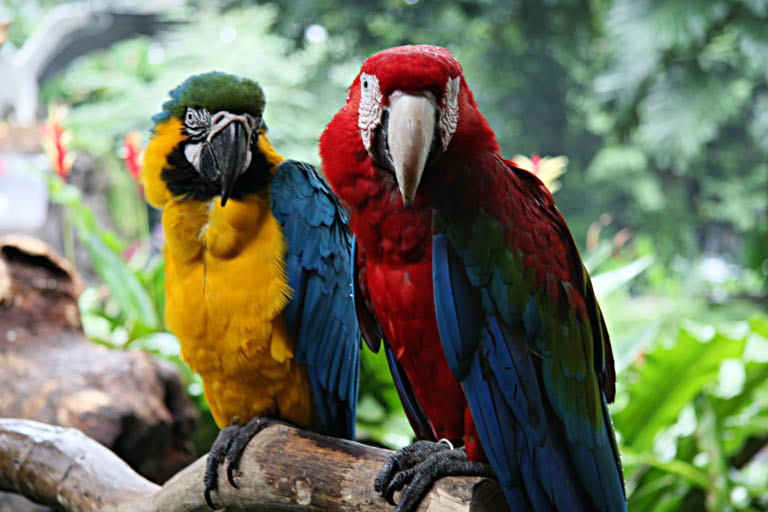
\includegraphics[width=.45\textwidth]{parrots.jpg}
\end{center}
You can download it at \url{https://raw.githubusercontent.com/parastuffs/4EISA-image-processing/main/Labo%201/parrots.bmp}, but really any image will do at this stage.

The \texttt{cv2.imread(file, mode)} method is used to import an image. It takes two arguments. The first argument \texttt{file} is the image filename. The image should either be in the same directory where the Python script is, or the absolute path should be provided to \texttt{cv2.imread()}. It reads images and saves it as a \numpy array.
The second argument is a flag which specifies the mode the image should be read in. The flag can have following values:
\begin{description}
\item[\texttt{cv2.IMREAD\_COLOR}] or 1: This loads a colour image. This is the default flag.
\item[\texttt{cv2.IMREAD\_GRAYSCALE}] or 0: This loads an image in greyscale mode.
\item[\texttt{cv2.IMREAD\_UNCHANGED}] or -1: This loads an image as it is, including the alpha channel.
\end{description}


Write following code in a new python script:
\begin{minted}{python}
#!/usr/bin/env python3
#This imports opencv
import cv2
#This reads and stores image in color into variable img
img = cv2.imread('parrots.bmp',cv2.IMREAD_COLOR)
img = cv2.imread('parrots.bmp',1)
\end{minted}
The last two lines are doing exactly the same thing.

The following code is used to display an image\footnote{Don't forget the shebang and to import \texttt{cv2}}:
\begin{minted}{python}
cv2.imshow('Parrots',img)
cv2.waitKey(0)
cv2.destroyWindow('Parrots')
\end{minted}

The \texttt{cv2.imshow(window, image)} function is used to display an image. The first argument is a string, which is the window name, and the second argument is the variable that holds the image which is to be displayed.\\

The \texttt{cv2.waitKey(time)} function is a keyboard function. Its argument is the time in milliseconds.
The function waits for specified milliseconds for any keyboard key press. If 0 is passed, it waits indefinitely for a key press. It is the only method to fetch and handle events. We must use this after \texttt{cv2.imshow()}, otherwise we don't have enough time to see the image.\\

The \texttt{cv2.destroyWindow()} function takes a window name as a parameter and destroys that window. If we want to destroy all the windows in the current program, we can use \texttt{cv2.destoyAllWindows()}.\\

Now, you know how to import and display an image, it can be useful to save it.
The \texttt{cv2.imwrite(file, image)} method is used to save an image to a specific path. The first argument is the name of the file and the second is the variable pointing to the image we want to save.

\begin{minted}{python}
import cv2
img = cv2.imread('parrots.bmp',1)
cv2.imshow('Parrots',img)
cv2.waitKey(0)
cv2.imwrite('output.jpg',img)
cv2.destroyWindow('Parrots')
\end{minted}


\numpy was introduced at the step 1 as a powerful tool to manipulate arrays. To start, you can execute the following code:

\begin{minted}{python}
import cv2
import matplotlib.pyplot as plt
# Program to load a color image in gray scale and to display it using matplotlib
img = cv2.imread('parrots.bmp',0)
plt.imshow(img,cmap='gray')
plt.title('Parrots')
plt.xticks([])
plt.yticks([])
plt.show()
\end{minted}

\begin{leftbar}
Try again the code but without the argument \texttt{cmap=’gray’}. What happens to the parrots?
\end{leftbar}

The colours are all wrong because the \texttt{cv2.imread()} function of \opencv reads images and saves it as a \numpy array of Blue, Green, and Red (BGR) pixels.\\

However, \texttt{plt.imshow()} displays images in RGB format. So, if we read the image as it is with \texttt{cv2.imread()} and display it using \texttt{plt.imshow()}, the value of the Blue colour will be treated as the value of Red and vice versa by \texttt{plt.imshow()}, and it would display the image with distorted colours.\\

To remedy this issue, we need to convert the image read in the BGR format into an RGB array format by \texttt{cv2.imread()} so that \texttt{plt.imshow()} will be able to render it in a way that makes sense to us. We will use the \texttt{cv2.cvtColor()} function for this in the step 4 and not worry about it for the moment.\\

\opencv also has drawing functions to create dots, lines, rectangles, circles, \dots~  It can be combined with NumPy to display and operate on the shapes. To do so, import the necessary libraries with the following lines:

\begin{minted}{python}
import cv2
import numpy as np
\end{minted}

Set a background image, for instance 400x400 black background as (0,0,0) is the black colour, with this line:

\begin{minted}{python}
image = np.zeros((400,400,3), np.uint8)
\end{minted}

Here is some other examples of shapes:

\begin{minted}{python}
# Blue (255,0,0) rectangle with the bottom left corner at (20,20)
# and the top right at (60,60).
cv2.rectangle(image,(20,20),(60,60),(255,0,0),1)

# Green circle centered on (80,80) with a radius of 10.
cv2.circle(image,(80,80),10,(0,255,0),-1)

# Ellipse without any rotation, centered on (99,99)
# and major and minor axis length of 40 and 20.
cv2.ellipse(image,(99,99),(40,20),0,0,360,(128,128,128),-1)

# Generic polygon with four points.
points = np.array([[100,5],[125,30],[175,20],[185,10]], np.int32)
points = points.reshape((-1,1,2))
cv2.polylines(image,[points],True,(255,255,0))
\end{minted}

If you pass False as the third argument in the \texttt{polylines()} function, it would join all the points and would not print a closed shape.\\

We can also print text in the image with \texttt{cv2.putText()}. The following code adds text to the image with (80,180) as the bottom-left corner of the text and \texttt{HERSHEY\_DUPLEX2}\footnote{Explore the \href{https://docs.opencv.org/4.x/}{\opencv documentation} to find the other possible fonts.} as the font with the size of 1 and colour pink:

\begin{minted}{python}
cv2.putText(image,'Test',(80,180),cv2.FONT_HERSHEY_DUPLEX,1,(255,0,255))
\end{minted}

\begin{leftbar}
Take your time to get used to the environment and do your own draft.
\end{leftbar}











\section*{Step 3 – Using Picamera in Python}
Make sure the camera module is enabled, navigate through \texttt{Raspberry Menu $\rightarrow$ Preferences $\rightarrow$ Raspberry Pi Configuration $\rightarrow$ interfaces $\rightarrow$ camera enable} and reboot the board if you needed to enable it.

The following program quickly demonstrates the basic usage of the picamera module to capture a picture:
\begin{minted}{python}
import picamera
import time
with picamera.PiCamera() as cam:
	cam.resolution=(1024,768)
	cam.start_preview()
	time.sleep(5)
	cam.capture('test.jpg')
\end{minted}
We have to import time and picamera modules first. The \texttt{cam.start\_preview()} method starts the preview and \texttt{time.sleep(5)} waits for 5 seconds before \texttt{cam.capture()} captures and saves the image in the specified file.

There is an inbuilt function in picamera for time-lapse photography. Let's see its usage using the following program:

\begin{minted}{python}
import picamera
import time
with picamera.PiCamera() as cam:
	cam.resolution=(640,480)
	cam.start_preview()
	time.sleep(3)
	for count, imagefile in enumerate(cam.capture_continuous('image{counter:02d}.jpg')):
		print(f"Capturing and saving {imagefile}")
		time.sleep(1)
		if count == 10:
			break
\end{minted}
In the preceding code, \texttt{cam.capture\_continuous()} is used to capture the time-lapse sequence using the Pi camera module.\\

Now, we know how to capture an image. Let’s try to capture it as an array and display it with OpenCV through \texttt{cv2.imshow()}. Here are the lines to realise the process.

\begin{minted}{python}
import picamera
import picamera.array
import time
import cv2
with picamera.PiCamera() as camera:
	rawCap=picamera.array.PiRGBArray(camera)
	camera.start_preview()
	time.sleep(6)
	camera.capture(rawCap,format="bgr")
image=rawCap.array
cv2.imshow("Test",image)
cv2.waitKey(0)
cv2.destroyAllWindows()
\end{minted}





\section*{Step 4 -- Basic image processing}
First of all, to process an image it is interesting to know the properties of the image. to obtain them we simply need the following code:

\begin{minted}{python}
import cv2
img = cv2.imread('parrots.bmp',1)
print(img.shape)
print(img.size)
print(img.dtype)
\end{minted}

The \texttt{img.shape()} function returns the shape of an image, that is, its dimensions and the number of color channels (usually 3, corresponding to RGB).\\

Try modifying the preceding code to read the image in greyscale mode and observe the output of \texttt{img.shape}.\\

The \texttt{img.size} function returns the total number of pixels and \texttt{img.dtype} returns the image data type.
Surprisingly (or not), we can perform directly arithmetic operations on images with \opencv as it is an array.\\

Images must be of the same size for you to perform arithmetic operations on the images, and these operations are performed on individual pixels.

\begin{description}
	\item[\texttt{cv2.add(a, b)}] This function is used to add two images, where the images are passed as parameters.
	\item[\texttt{cv2.subtract(a, b)}] This function is used to subtract image \texttt{b} from image \texttt{a}.
\end{description}

Here is an example of use:
\begin{minted}{python}
import cv2
img1 = cv2.imread('parrots.bmp',1)
img2 = cv2.imread('another_img.bmp',1)
cv2.imshow('Image1',img1)
cv2.waitKey(0)
cv2.imshow('Image2',img2)
cv2.waitKey(0)
cv2.imshow('Addition',cv2.add(img1,img2))
cv2.waitKey(0)
cv2.imshow('Image1-Image2',cv2.subtract(img1,img2))
cv2.waitKey(0)
cv2.imshow('Image2-Image1',cv2.subtract(img2,img1))
cv2.waitKey(0)
cv2.destroyAllWindows()
\end{minted}

Like Whiskies, you can also blend your images. The \texttt{cv2.addWeighted()} function calculates the weighted sum of two images. Because of the weight factor, it provides a blending effect to the images. Add the following lines of code before \texttt{destroyAllWindows()} in the previous code listing to see this function in action:

\begin{minted}{python}
cv2.addWeighted(img1,0.5,img2,0.5,0)
cv2.waitKey(0)
\end{minted}
In the preceding code, we passed the following five arguments to the \texttt{addWeighted()} function:
\begin{description}
	\item[\texttt{Img1}] first image
	\item[\texttt{Alpha}]  weight factor for the first image (0.5 in the example)
	\item[\texttt{Img2}]  second image
	\item[\texttt{Beta}] weight factor for the second image (0.5 in the example)
	\item[\texttt{Gamma}]  scalar offset value (0 in the example)
\end{description}

The output image value is calculated with the following formula:
\[\text{Output}=(\alpha*\text{\texttt{img1}})+(\beta*\text{\texttt{img2}})+\gamma\]

This operation is performed on every individual pixel.

We can create a film-style transition effect on the two images by using the same function. Check out the output of the following code that creates a smooth image transition from an image to another image:

\begin{minted}{python}
import cv2
import numpy as np
import time
img1 = cv2.imread('parrots.bmp',1)
img2 = cv2.imread('another_img.bmp',1)
for i in np.linspace(0,1,40):
	alpha = i
	beta = 1-alpha
	print(f"ALPHA = {alpha}, BETA = {beta}")
	cv2.imshow('Image Transition',
	cv2.addWeighted(img1,alpha,img2,beta,0))
	time.sleep(0.05)
	if cv2.waitKey(1) == 27 :
		break
cv2.destroyAllWindows()
\end{minted}

On several occasions, we may be interested in working separately with the red, green, and blue channels. For example, we might want to build a histogram for every channel of an image. Here, \texttt{cv2.split()} is used to split an image into three different intensity arrays for each colour channel, whereas \texttt{cv2.merge()} is used to merge different arrays into a single multi- channel array, that is, a colour image. The following example demonstrates this:

\begin{minted}{python}
import cv2
img = cv2.imread('parrots.bmp',1)
b,g,r = cv2.split(img)
cv2.imshow('Blue Channel', b)
cv2.imshow('Green Channel', g)
cv2.imshow('Red Channel', r)
img = cv2.merge((b,g,r))
cv2.imshow('Merged Output', img)
cv2.waitKey(0)
cv2.destroyAllWindows()
\end{minted}
The preceding program first splits the image into three channels (blue, green, and red) and then displays each one of them. The separate channels will only hold the intensity values of the particular colour and the images will essentially be displayed as greyscale intensity images. Then, the program merges all the channels back into an image and displays it.


\subsection*{Creating a negative of an image}
In mathematical terms, the negative of an image is the inversion of colours. For a greyscale image, it is even simpler! The negative of a greyscale image is just the intensity inversion, which can be achieved by finding the complement of the intensity from 255. A pixel value ranges from 0 to 255, and therefore, negation involves the subtracting of the pixel value from the maximum value, that is, 255. The code for the same is as follows:

\begin{minted}{python}
import cv2
img = cv2.imread('parrots.bmp')
grayscale = cv2.cvtColor(img,cv2.COLOR_BGR2GRAY)
negative = abs(255-grayscale)
cv2.imshow('Original',img)
cv2.imshow('Grayscale',grayscale)
cv2.imshow('Negative',negative)
cv2.waitKey(0)
cv2.destroyAllWindows()
\end{minted}


\subsection*{Logical operations on images}
OpenCV provides bitwise logical operation functions for images. We will have a look at the functions that provide the bitwise logical AND, OR, XOR (exclusive OR), and NOT (inversion) functionality. These functions can be better demonstrated visually with greyscale images. We will use barcode images in horizontal and vertical orientation for demonstration.\\

Let's have a look at the following code:

\begin{minted}{python}
import cv2
import matplotlib.pyplot as plt
img1 = cv2.imread('Barcode_Hor.png',0)
img2 = cv2.imread('Barcode_Ver.png',0)
not_out=cv2.bitwise_not(img1)
and_out=cv2.bitwise_and(img1,img2)
or_out=cv2.bitwise_or(img1,img2)
xor_out=cv2.bitwise_xor(img1,img2)
titles = ['Image 1','Image 2','Image 1 NOT','AND','OR','XOR']
images = [img1,img2,not_out,and_out,or_out,xor_out]
for i in xrange(6):
	plt.subplot(2,3,i+1)
	plt.imshow(images[i],cmap='gray')
	plt.title(titles[i])
	plt.xticks([]),plt.yticks([])
plt.show()
\end{minted}

We first read the images in greyscale mode and calculated the NOT, AND, OR, and XOR, functionalities and then with \texttt{matplotlib}, we displayed those in a neat way. We leveraged the \texttt{mplt.subplot()} function to display multiple images. Here in the preceding example, we created a grid with two rows and three columns for our images and displayed each image in every part of the grid. You can modify this line and change it to \texttt{mplt.subplot(3,2,i+1)} to create a grid with three rows and two columns. We will use this technique heavily throughout the book to display images side-by-side or in a grid.\\

You may want to have a look at the functionality of \texttt{cv2.copyMakeBorder()}. This function is used to create the borders and paddings for images, and many of you will find it useful for your projects.




\section*{Challenge}
For this part you are free to experience any program with \opencv and the PiCamera.
Navigate on the \opencv API: \url{https://docs.opencv.org/4.x/} and the PiCamera documentation: \url{https://picamera.readthedocs.io/}.\\

As a good start try to take a picture of the EuroRobot Playground and isolate the different area of the player 1 and player 2. Then find a way to isolate the different pathways.
Your challenge is to analyse the playground in depth and to obtain as much information as possible from it.



%\Question{}{}
\end{document}
